% ============================================================
% Material expandido - Semana 5 - Aplicaciones Distribuidas (ISR-701)
% Unidad 2: Arquitecturas Distribuidas
% Tema 3: Contenedores y Orquestacion de Servicios
% UTEQ - Facultad de Ciencias de la Computacion y Diseno Digital
% ============================================================
\documentclass[11pt,a4paper]{article}

\usepackage[utf8]{inputenc}
\usepackage[T1]{fontenc}
\usepackage[scaled=0.96]{helvet}
\renewcommand{\familydefault}{\sfdefault}
\usepackage[a4paper,margin=2.3cm,headheight=15pt]{geometry}
\usepackage{microtype}
\usepackage{xcolor}
\usepackage{graphicx}
\usepackage{booktabs}
\usepackage{array}
\usepackage{tabularx}
\usepackage{ragged2e}
\usepackage{enumitem}
\usepackage{amsmath}
\usepackage{amssymb}
\usepackage[most]{tcolorbox}
\usepackage{listings}
\usepackage{listingsutf8}
\usepackage{fancyhdr}
\usepackage{titlesec}
\usepackage{tikz}
\usetikzlibrary{positioning,arrows.meta,shapes.geometric,calc,fit,backgrounds}
\usepackage[hidelinks]{hyperref}
\hypersetup{colorlinks=true,linkcolor=uteqBlue,urlcolor=uteqTeal,citecolor=uteqMid}

% ---------------- Paleta UTEQ ----------------
\definecolor{uteqBlue}{RGB}{31,56,100}     % azul oscuro
\definecolor{uteqMid}{RGB}{46,94,170}      % azul medio
\definecolor{uteqTeal}{RGB}{15,140,140}    % teal
\definecolor{uteqGreen}{RGB}{0,127,71}     % verde institucional
\definecolor{uteqAmber}{RGB}{200,120,0}    % ambar (advertencia)
\definecolor{grayBg}{RGB}{244,246,249}
\definecolor{grayLine}{RGB}{210,216,224}
\definecolor{codeBg}{RGB}{248,249,251}
\definecolor{codeKw}{RGB}{20,80,160}
\definecolor{codeCm}{RGB}{96,120,96}
\definecolor{codeStr}{RGB}{160,70,30}

% ---------------- Encabezado / pie ----------------
\pagestyle{fancy}
\fancyhf{}
\renewcommand{\headrulewidth}{0.8pt}
\renewcommand{\footrulewidth}{0.4pt}
\fancyhead[L]{\footnotesize\textcolor{uteqBlue}{\textbf{UTEQ} \textbar{} Ing. de Software}}
\fancyhead[R]{\footnotesize\textcolor{uteqBlue}{Aplicaciones Distribuidas \textbar{} Semana 5}}
\fancyfoot[L]{\footnotesize Unidad 2 - Tema 3: Contenedores y Orquestaci\'on}
\fancyfoot[C]{\footnotesize\textcolor{uteqMid}{Prof. Guerrero Ulloa G.C.}}
\fancyfoot[R]{\footnotesize\thepage}

% ---------------- Titulos ----------------
\titleformat{\section}{\Large\bfseries\color{uteqBlue}}{\thesection.}{0.5em}{}
\titleformat{\subsection}{\large\bfseries\color{uteqMid}}{\thesubsection.}{0.5em}{}
\titleformat{\subsubsection}{\normalsize\bfseries\color{uteqTeal}}{\thesubsubsection.}{0.5em}{}
\titlespacing*{\section}{0pt}{12pt}{6pt}

% ---------------- Cajas tcolorbox ----------------
\newtcolorbox{defbox}[1][]{colback=uteqTeal!6,colframe=uteqTeal,boxrule=0.9pt,arc=2pt,
  left=8pt,right=8pt,top=6pt,bottom=6pt,fonttitle=\bfseries\color{white},
  coltitle=white,colbacktitle=uteqTeal,title={#1}}
\newtcolorbox{keybox}[1][]{colback=uteqBlue!5,colframe=uteqBlue,boxrule=0.9pt,arc=2pt,
  left=8pt,right=8pt,top=6pt,bottom=6pt,fonttitle=\bfseries\color{white},
  coltitle=white,colbacktitle=uteqBlue,title={#1}}
\newtcolorbox{ideabox}[1][]{colback=uteqMid!6,colframe=uteqMid,boxrule=0.9pt,arc=2pt,
  left=8pt,right=8pt,top=6pt,bottom=6pt,fonttitle=\bfseries\color{white},
  coltitle=white,colbacktitle=uteqMid,title={#1}}
\newtcolorbox{warnbox}[1][]{colback=uteqAmber!8,colframe=uteqAmber,boxrule=0.9pt,arc=2pt,
  left=8pt,right=8pt,top=6pt,bottom=6pt,fonttitle=\bfseries\color{white},
  coltitle=white,colbacktitle=uteqAmber,title={#1}}

% ---------------- Macro para nombre de archivo ----------------
\newcommand{\archivo}[1]{\par\vspace{5pt}\noindent\colorbox{uteqBlue}{\textcolor{white}{\small\,\faFileIco\ \texttt{#1}\,}}\par\nopagebreak\vspace{1pt}}
\newcommand{\faFileIco}{\raisebox{-0.1ex}{\scriptsize$\square$}}

% ---------------- Estilos de codigo ----------------
\lstset{
  basicstyle=\ttfamily\footnotesize,
  backgroundcolor=\color{codeBg},
  frame=single,
  framesep=5pt,
  rulecolor=\color{grayLine},
  keywordstyle=\color{codeKw}\bfseries,
  commentstyle=\color{codeCm}\itshape,
  stringstyle=\color{codeStr},
  numbers=left,
  numberstyle=\tiny\color{gray},
  numbersep=8pt,
  showstringspaces=false,
  breaklines=true,
  breakatwhitespace=true,
  tabsize=2,
  columns=fullflexible,
  keepspaces=true,
  upquote=true,
  literate={~}{{\textasciitilde}}1
}

\lstdefinelanguage{Dockerfile}{
  keywords={FROM,AS,RUN,CMD,COPY,ADD,WORKDIR,EXPOSE,ENV,ENTRYPOINT,USER,LABEL,ARG,VOLUME,HEALTHCHECK},
  keywordstyle=\color{codeKw}\bfseries,
  morecomment=[l]{\#},
  morestring=[b]",
  sensitive=true
}
\lstdefinelanguage{yaml}{
  keywords={true,false,null},
  keywordstyle=\color{codeKw},
  morecomment=[l]{\#},
  morestring=[b]",
  basicstyle=\ttfamily\footnotesize,
  sensitive=true
}
\lstdefinelanguage{properties}{
  morecomment=[l]{\#},
  morestring=[b]",
  sensitive=true
}
\lstdefinelanguage{nginxconf}{
  keywords={server,location,upstream,listen,proxy_pass,proxy_set_header,limit_req,limit_req_zone,access_log,error_log},
  keywordstyle=\color{codeKw}\bfseries,
  morecomment=[l]{\#},
  sensitive=true
}

% ---------------- Numeracion de tablas/figuras ----------------
\renewcommand{\arraystretch}{1.25}
\setlist{itemsep=2pt,topsep=3pt,parsep=0pt}
\setlength{\emergencystretch}{3em}
\newcolumntype{C}{>{\Centering\arraybackslash}X}
\renewcommand{\figurename}{Figura}
\renewcommand{\tablename}{Tabla}
\renewcommand{\refname}{Referencias}


\begin{document}

% ===================== PORTADA =====================
\begin{center}
{\color{uteqGreen}\rule{\textwidth}{3pt}}\\[2pt]
{\large\textbf{\textcolor{uteqBlue}{UNIVERSIDAD T\'ECNICA ESTATAL DE QUEVEDO}}}\\[2pt]
{\small Facultad de Ciencias de la Computaci\'on y Dise\~no Digital \textbar{} Carrera de Ingenier\'ia de Software}\\[4pt]
{\color{uteqGreen}\rule{\textwidth}{1.2pt}}\\[10pt]
{\LARGE\textbf{\textcolor{uteqBlue}{Material de Clase --- Semana 5}}}\\[6pt]
{\Large\textbf{\textcolor{uteqMid}{Contenedores y Orquestaci\'on de Servicios}}}\\[10pt]
\end{center}

\begin{keybox}[Datos de la semana]
\begin{tabularx}{\linewidth}{@{}>{\bfseries}l X@{}}
Asignatura & Aplicaciones Distribuidas (ISR-701) --- S\'eptimo semestre \\
Unidad & 2: Arquitecturas Distribuidas \\
Tema & 3: Contenedores y Orquestaci\'on de Servicios \\
Semana & 5 de 18 \quad\textbar\quad Fechas: 01 -- 07 de junio de 2026 \\
Subtemas & (1) Virtualizaci\'on y contenerizaci\'on: Docker; (2) Composici\'on de servicios: Docker Compose; (3) Introducci\'on a Kubernetes: pods, deployments y services; (4) Patrones de despliegue distribuido (blue-green, canary) \\
Docente & Prof. Guerrero Ulloa G.C. \\
\end{tabularx}
\end{keybox}

\begin{defbox}[Resultado de aprendizaje de la unidad]
Aplica arquitecturas y patrones de dise\~no distribuido ---microservicios, API REST, mensajer\'ia as\'incrona, arquitectura en capas--- para construir sistemas \textbf{escalables}, \textbf{disponibles} y \textbf{seguros}. Esta semana operacionaliza ese resultado: empaquetar el microservicio en un \emph{artefacto inmutable} (imagen), componer el sistema completo de forma reproducible y orquestarlo con tolerancia a fallos y despliegues sin interrupci\'on.
\end{defbox}

\begin{warnbox}[Nota de coherencia curricular]
El temario de esta semana corresponde, en el libro gu\'ia (Guerrero Ulloa, 2026), al \textbf{Cap\'itulo 7: ``Contenedores Docker y Orquestaci\'on''}. La numeraci\'on de cap\'itulos del libro avanza tema a tema; el \emph{cronograma} de la asignatura agrupa Docker, Compose y Kubernetes como Tema 3 de la Unidad 2 (Arquitecturas Distribuidas), que es el orden seguido aqu\'i. El microservicio de ejemplo, \texttt{svc-estudiantes}, es el mismo construido en la semana previa (Spring Boot + Java), de modo que esta clase lo \emph{empaqueta y despliega} sin re-escribir l\'ogica de negocio.
\end{warnbox}

\section{Mapa de la semana y objetivos operativos}

Las tres semanas de la Unidad 2 trazan una progresi\'on natural: primero se decide \emph{c\'omo se estructura} el sistema (monolito a microservicios), luego \emph{c\'omo se comunican} sus partes (APIs REST) y, finalmente ---esta semana---, \emph{c\'omo se empaqueta, se compone y se despliega} ese sistema en m\'aquinas reales con garant\'ias de disponibilidad. El hilo conductor es la palabra \textbf{reproducibilidad}: el mismo artefacto debe ejecutarse id\'entico en la laptop del estudiante, en el laboratorio y en un servidor de producci\'on.

Al finalizar la semana, el estudiante ser\'a capaz de: (i) explicar por qu\'e los contenedores resuelven el problema ``en mi m\'aquina funciona'' mejor que las m\'aquinas virtuales; (ii) escribir un \texttt{Dockerfile} multi-etapa correcto y construir una imagen del microservicio desde IntelliJ IDEA; (iii) componer el sistema (microservicio + base de datos + gateway) con un \'unico archivo \texttt{compose.yaml}; (iv) desplegar ese sistema en un cl\'uster Kubernetes describiendo \texttt{Deployments} y \texttt{Services}; y (v) razonar sobre los patrones \emph{blue-green} y \emph{canary} para liberar versiones nuevas sin tiempo de ca\'ida.

\begin{ideabox}[Glosario de acr\'onimos usados en la semana]
\textbf{VM} Virtual Machine (m\'aquina virtual) \textbullet{} \textbf{SO} Sistema Operativo \textbullet{} \textbf{CLI} Command-Line Interface \textbullet{} \textbf{JDK} Java Development Kit \textbullet{} \textbf{JRE} Java Runtime Environment \textbullet{} \textbf{JAR} Java ARchive \textbullet{} \textbf{API} Application Programming Interface \textbullet{} \textbf{REST} Representational State Transfer \textbullet{} \textbf{YAML} YAML Ain't Markup Language \textbullet{} \textbf{IDE} Integrated Development Environment \textbullet{} \textbf{K8s} Kubernetes \textbullet{} \textbf{Pod} unidad m\'inima de despliegue en K8s \textbullet{} \textbf{etcd} almac\'en clave-valor del plano de control \textbullet{} \textbf{PVC} PersistentVolumeClaim \textbullet{} \textbf{CRD} Custom Resource Definition \textbullet{} \textbf{SLA} Service Level Agreement.
\end{ideabox}

% ===================================================================
\section{Subtema 1 --- Virtualizaci\'on y contenerizaci\'on: Docker}

\subsection{El problema que resuelve un contenedor}

Todo desarrollador ha vivido el s\'indrome ``en mi m\'aquina funciona''. Ocurre porque una aplicaci\'on no depende solo de su c\'odigo, sino de un \emph{entorno}: versi\'on exacta del runtime (por ejemplo Java 25), variables de entorno, librer\'ias del sistema, configuraci\'on de red y rutas de archivos. Cuando ese entorno difiere entre la laptop, el laboratorio y el servidor, el comportamiento diverge. La \textbf{contenerizaci\'on} ataca el problema de ra\'iz: empaqueta la aplicaci\'on \emph{junto con todas sus dependencias} en una unidad est\'andar y port\'atil llamada \textbf{imagen}, que se ejecuta de forma id\'entica en cualquier host con un motor de contenedores instalado.

\begin{defbox}[Definici\'on: contenedor]
Un \textbf{contenedor} es un proceso (o conjunto de procesos) aislado del resto del sistema mediante primitivas del n\'ucleo de Linux ---\emph{namespaces} (aislamiento de visi\'on: procesos, red, montajes) y \emph{cgroups} (control de recursos: CPU, memoria, E/S)---, que comparte el \textbf{n\'ucleo del sistema operativo anfitri\'on} en lugar de virtualizar hardware completo. Esto lo hace ligero (megabytes, no gigabytes), de arranque casi instant\'aneo y reproducible \cite{merkel2014,bernstein2014}.
\end{defbox}

\subsection{M\'aquinas virtuales frente a contenedores}

La diferencia esencial es \emph{qu\'e} se virtualiza. Una m\'aquina virtual virtualiza \textbf{hardware} mediante un hipervisor y ejecuta un sistema operativo invitado completo por cada instancia; un contenedor virtualiza el \textbf{sistema operativo} y reutiliza el n\'ucleo del anfitri\'on. La consecuencia pr\'actica es enorme: donde un servidor aloja una decena de VMs, puede alojar cientos de contenedores, con tiempos de arranque que pasan de minutos a milisegundos \cite{pahl2019}.

\begin{figure}[h]
\centering
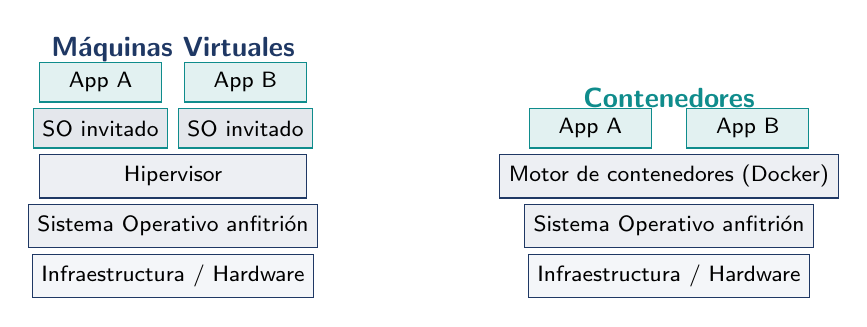
\begin{tikzpicture}[font=\footnotesize,
  layer/.style={draw=uteqBlue,fill=uteqBlue!8,minimum width=3.4cm,minimum height=0.55cm,align=center},
  appl/.style={draw=uteqTeal,fill=uteqTeal!12,minimum width=1.55cm,minimum height=0.5cm,align=center}]
% --- VM stack ---
\node[layer,fill=grayBg] (vmh) at (0,0) {Infraestructura / Hardware};
\node[layer,above=2pt of vmh] (vmhost) {Sistema Operativo anfitri\'on};
\node[layer,above=2pt of vmhost] (vmhyp) {Hipervisor};
\node[appl,above=2pt of vmhyp,xshift=-0.92cm,fill=uteqBlue!12] (vmg1) {SO invitado};
\node[appl,above=2pt of vmhyp,xshift=0.92cm,fill=uteqBlue!12] (vmg2) {SO invitado};
\node[appl,above=2pt of vmg1] (vma1) {App A};
\node[appl,above=2pt of vmg2] (vma2) {App B};
\node[above=4pt of $(vma1)!0.5!(vma2)$,font=\bfseries\color{uteqBlue}] {M\'aquinas Virtuales};
% --- Container stack ---
\begin{scope}[xshift=6.3cm]
\node[layer,fill=grayBg] (ch) at (0,0) {Infraestructura / Hardware};
\node[layer,above=2pt of ch] (chost) {Sistema Operativo anfitri\'on};
\node[layer,above=2pt of chost] (ceng) {Motor de contenedores (Docker)};
\node[appl,above=2pt of ceng,xshift=-1.0cm] (ca1) {App A};
\node[appl,above=2pt of ceng,xshift=1.0cm] (ca2) {App B};
\node[above=4pt of $(ca1)!0.5!(ca2)$,font=\bfseries\color{uteqTeal}] {Contenedores};
\end{scope}
\end{tikzpicture}
\caption{La VM duplica un sistema operativo invitado por instancia; el contenedor comparte el n\'ucleo del anfitri\'on, eliminando esa capa pesada.}
\label{fig:vmvscont}
\end{figure}

\begin{table}[h]
\centering
\caption{Comparaci\'on cuantitativa orientativa entre m\'aquinas virtuales y contenedores.}
\label{tab:vmvscont}
\small
\begin{tabularx}{\linewidth}{@{}l C C@{}}
\toprule
\textbf{Criterio} & \textbf{M\'aquina Virtual} & \textbf{Contenedor} \\
\midrule
Unidad virtualizada & Hardware (SO invitado completo) & Sistema operativo (comparte n\'ucleo) \\
Tama\~no t\'ipico & Gigabytes & Decenas de megabytes \\
Arranque & Decenas de segundos a minutos & Milisegundos a segundos \\
Densidad por host & Decenas & Cientos \\
Aislamiento & Fuerte (frontera de hardware) & Bueno (namespaces/cgroups) \\
Caso de uso ideal & Cargas heterog\'eneas / SO distintos & Microservicios homog\'eneos y escalables \\
\bottomrule
\end{tabularx}
\end{table}

\subsection{Arquitectura de Docker}

Docker implementa una arquitectura \textbf{cliente-servidor}. El \textbf{cliente} (\texttt{docker} en la CLI o la integraci\'on de IntelliJ) env\'ia \'ordenes; el \textbf{Docker daemon} (\texttt{dockerd}) las ejecuta: construye im\'agenes, crea contenedores y gestiona redes y vol\'umenes. Las piezas que el estudiante debe distinguir con precisi\'on son cuatro.

\begin{itemize}
\item \textbf{Imagen (image):} plantilla inmutable, de solo lectura, organizada en capas. Cada instrucci\'on del \texttt{Dockerfile} a\~nade una capa cacheable. Es el ``molde''.
\item \textbf{Contenedor (container):} instancia en ejecuci\'on de una imagen, con una capa de escritura ef\'imera encima. Es el ``objeto'' creado a partir del molde.
\item \textbf{Dockerfile:} receta de texto que describe c\'omo construir la imagen, paso a paso.
\item \textbf{Registro (registry):} repositorio de im\'agenes (Docker Hub, GitHub Container Registry). \texttt{docker pull} descarga y \texttt{docker push} publica.
\end{itemize}

\subsection{El Dockerfile y sus instrucciones esenciales}

Un \texttt{Dockerfile} es una secuencia de instrucciones; cada una genera una capa. Conviene memorizar el n\'ucleo: \texttt{FROM} (imagen base), \texttt{WORKDIR} (directorio de trabajo), \texttt{COPY} (copia archivos al contexto de la imagen), \texttt{RUN} (ejecuta un comando en tiempo de construcci\'on), \texttt{EXPOSE} (documenta el puerto), \texttt{ENV} (variables de entorno), \texttt{USER} (usuario de ejecuci\'on) y \texttt{ENTRYPOINT}/\texttt{CMD} (proceso que arranca el contenedor). La diferencia entre \texttt{ENTRYPOINT} y \texttt{CMD} es sutil pero examinable: \texttt{ENTRYPOINT} define el ejecutable fijo; \texttt{CMD} aporta argumentos por defecto que el usuario puede sobrescribir.

\begin{keybox}[Construcci\'on multi-etapa: por qu\'e importa]
Compilar Java requiere el \textbf{JDK} (cientos de megabytes); ejecutar el \texttt{.jar} solo requiere el \textbf{JRE}. Una construcci\'on \emph{multi-stage} usa una etapa pesada para compilar y copia \'unicamente el artefacto final a una etapa de runtime ligera. Resultado: la imagen publicada es peque\~na, arranca r\'apido y reduce la superficie de ataque (menos software = menos vulnerabilidades).
\end{keybox}

\subsection{Estructura de archivos del proyecto (etapa Docker)}

El microservicio \texttt{svc-estudiantes} (Spring Boot 4.0.x sobre Java 25) ya existe de la semana anterior. Para contenerizarlo se a\~naden dos archivos en la ra\'iz: el \texttt{Dockerfile} y el \texttt{.dockerignore}.

\begin{lstlisting}[basicstyle=\ttfamily\footnotesize,numbers=none]
svc-estudiantes/
|-- mvnw                         # wrapper de Maven (Linux/macOS)
|-- mvnw.cmd                     # wrapper de Maven (Windows)
|-- pom.xml                      # dependencias y build
|-- Dockerfile                   # <-- NUEVO: receta de la imagen
|-- .dockerignore                # <-- NUEVO: que NO copiar al contexto
|-- .mvn/wrapper/                # binarios del wrapper
`-- src/
    `-- main/
        |-- java/ec/edu/uteq/svcestudiantes/
        |   |-- SvcEstudiantesApplication.java
        |   |-- controller/EstudianteController.java
        |   |-- service/EstudianteService.java
        |   |-- repository/EstudianteRepository.java
        |   |-- model/Estudiante.java
        |   `-- dto/EstudianteDTO.java
        `-- resources/
            |-- application.properties
            `-- application-docker.properties   # <-- NUEVO: perfil contenedor
\end{lstlisting}

\archivo{svc-estudiantes/Dockerfile}
\begin{lstlisting}[language=Dockerfile]
# syntax=docker/dockerfile:1

# ===== Etapa 1: build (pesada, con JDK) =====
FROM eclipse-temurin:25-jdk AS build
WORKDIR /workspace

# Copiar primero el wrapper y el pom para cachear dependencias
COPY .mvn/ .mvn/
COPY mvnw pom.xml ./
RUN chmod +x mvnw && ./mvnw -q -B dependency:go-offline

# Copiar el codigo fuente y empaquetar (sin tests para acelerar la imagen)
COPY src ./src
RUN ./mvnw -q -B clean package -DskipTests

# ===== Etapa 2: runtime (ligera, solo JRE) =====
FROM eclipse-temurin:25-jre-alpine AS runtime
WORKDIR /app

# Usuario sin privilegios (buena practica de seguridad)
RUN addgroup -S app && adduser -S app -G app

# Copiar SOLO el artefacto final desde la etapa de build
COPY --from=build /workspace/target/*.jar app.jar

EXPOSE 8080
USER app
ENTRYPOINT ["java", "-jar", "/app/app.jar"]
\end{lstlisting}

\archivo{svc-estudiantes/.dockerignore}
\begin{lstlisting}[numbers=none]
target/
.git/
.idea/
*.iml
*.log
.env
\end{lstlisting}

\archivo{svc-estudiantes/src/main/resources/application-docker.properties}
\begin{lstlisting}[language=properties]
# Perfil activo cuando el microservicio corre dentro de un contenedor.
# Los valores llegan por variables de entorno (12-factor app).
server.port=8080
spring.datasource.url=${SPRING_DATASOURCE_URL}
spring.datasource.username=${SPRING_DATASOURCE_USERNAME}
spring.datasource.password=${SPRING_DATASOURCE_PASSWORD}
spring.jpa.hibernate.ddl-auto=update
# Endpoints de salud para sondas de Compose y Kubernetes:
management.endpoints.web.exposure.include=health,info,prometheus
management.endpoint.health.probes.enabled=true
\end{lstlisting}

\subsection{Paso a paso en IntelliJ IDEA}

\begin{enumerate}
\item \textbf{Conectar el daemon.} Instale y arranque Docker Desktop (Windows/macOS) o el Docker Engine (Linux/WSL2). En IntelliJ: \emph{Settings} $\rightarrow$ \emph{Build, Execution, Deployment} $\rightarrow$ \emph{Docker} $\rightarrow$ \textbf{+} y seleccione \emph{Docker for Windows} / \emph{Unix socket}. Un punto verde confirma la conexi\'on.
\item \textbf{Crear el Dockerfile.} Clic derecho sobre la ra\'iz del proyecto $\rightarrow$ \emph{New} $\rightarrow$ \emph{File} $\rightarrow$ \texttt{Dockerfile}. IntelliJ reconoce el tipo y ofrece autocompletado de instrucciones.
\item \textbf{Construir la imagen.} En el margen izquierdo (gutter) del editor, junto a la l\'inea \texttt{FROM}, aparece un icono de \emph{play} doble: \emph{Build Image\ldots}. Asigne la etiqueta \texttt{svc-estudiantes:1.0.0}.
\item \textbf{Verla y ejecutarla.} Abra la ventana \emph{Services} (\emph{View} $\rightarrow$ \emph{Tool Windows} $\rightarrow$ \emph{Services}). Bajo el nodo \emph{Docker} ver\'a \emph{Images} y \emph{Containers}. Clic derecho sobre la imagen $\rightarrow$ \emph{Run\ldots}, mapee el puerto \texttt{8080:8080}.
\item \textbf{Inspeccionar.} En \emph{Services}, seleccione el contenedor para ver \emph{Logs}, \emph{Environment}, \emph{Files} y abrir una terminal con \emph{Exec} $\rightarrow$ \texttt{/bin/sh}.
\end{enumerate}

\begin{ideabox}[Comandos equivalentes en terminal]
Para quienes prefieren la CLI (PowerShell por defecto; Linux/macOS como comentario):
\end{ideabox}

\archivo{Terminal --- Windows PowerShell}
\begin{lstlisting}[numbers=none]
# Construir la imagen desde la raiz del proyecto
docker build -t svc-estudiantes:1.0.0 .
# Linux/macOS: identico

# Ejecutar el contenedor publicando el puerto
docker run --rm -p 8080:8080 svc-estudiantes:1.0.0

# Probar el endpoint de salud (PowerShell usa curl.exe, no el alias)
curl.exe http://localhost:8080/actuator/health
# Linux/macOS:  curl http://localhost:8080/actuator/health

# Listar imagenes y contenedores; ver consumo
docker images
docker ps
docker stats --no-stream
\end{lstlisting}

\begin{warnbox}[Errores t\'ipicos que penalizan en la pr\'actica]
(1) Copiar todo el proyecto antes del \texttt{pom.xml}: rompe la cach\'e de capas y cada cambio recompila dependencias. (2) Usar la imagen JDK en runtime: imagen innecesariamente enorme. (3) Ejecutar como \texttt{root}: falla de seguridad. (4) Olvidar \texttt{.dockerignore}: se copia \texttt{target/} y \texttt{.git/}, inflando el contexto de construcci\'on.
\end{warnbox}

% ===================================================================
\section{Subtema 2 --- Composici\'on de servicios: Docker Compose}

\subsection{Por qu\'e Compose}

Un microservicio rara vez vive solo: necesita una base de datos, quiz\'a un gateway, una cach\'e. Levantar cada pieza con \texttt{docker run} y conectarlas a mano es fr\'agil y no reproducible. \textbf{Docker Compose} resuelve esto con un \'unico archivo declarativo, \texttt{compose.yaml}, que describe \emph{todos} los servicios, sus redes y vol\'umenes; un solo comando, \texttt{docker compose up}, levanta el sistema completo en el orden correcto.

\begin{defbox}[Modelo declarativo]
En lugar de decir \emph{c\'omo} arrancar cada contenedor (imperativo), se declara el \textbf{estado deseado} del sistema (declarativo) y Compose lo materializa. Este es el mismo principio que rige Kubernetes; dominarlo aqu\'i facilita el salto al subtema siguiente.
\end{defbox}

\subsection{Anatom\'ia de \texttt{compose.yaml}}

Las claves esenciales son: \texttt{services} (cada contenedor del sistema), \texttt{image}/\texttt{build} (de d\'onde sale su imagen), \texttt{environment} (variables), \texttt{ports} (publicaci\'on al host), \texttt{expose} (visibilidad solo interna), \texttt{depends\_on} (orden y, con \texttt{condition}, espera de salud), \texttt{healthcheck} (sonda de disponibilidad), \texttt{volumes} (persistencia) y \texttt{networks} (segmentaci\'on). Desde la especificaci\'on actual de Compose ya \textbf{no se escribe} la clave \texttt{version}.

\subsection{Estructura de archivos del proyecto (etapa Compose)}

\begin{lstlisting}[basicstyle=\ttfamily\footnotesize,numbers=none]
svc-estudiantes/
|-- Dockerfile
|-- .dockerignore
|-- compose.yaml            # <-- NUEVO: orquestacion local del stack
|-- .env.example           # <-- NUEVO: plantilla de variables (sin secretos)
|-- infra/
|   `-- nginx/
|       `-- nginx.conf      # <-- NUEVO: configuracion del API Gateway
`-- src/ ...
\end{lstlisting}

\archivo{svc-estudiantes/compose.yaml}
\begin{lstlisting}[language=yaml]
name: svc-estudiantes-stack

services:
  db:
    image: postgres:17-alpine
    environment:
      POSTGRES_DB: ${POSTGRES_DB}
      POSTGRES_USER: ${POSTGRES_USER}
      POSTGRES_PASSWORD: ${POSTGRES_PASSWORD}
    volumes:
      - db-data:/var/lib/postgresql/data
    healthcheck:
      test: ["CMD-SHELL", "pg_isready -U ${POSTGRES_USER} -d ${POSTGRES_DB}"]
      interval: 10s
      timeout: 5s
      retries: 5
    networks: [backend]

  app:
    build: .
    image: svc-estudiantes:1.0.0
    environment:
      SPRING_PROFILES_ACTIVE: docker
      SPRING_DATASOURCE_URL: jdbc:postgresql://db:5432/${POSTGRES_DB}
      SPRING_DATASOURCE_USERNAME: ${POSTGRES_USER}
      SPRING_DATASOURCE_PASSWORD: ${POSTGRES_PASSWORD}
    depends_on:
      db:
        condition: service_healthy   # espera a que la BD este sana
    expose: ["8080"]                 # visible solo en la red interna
    networks: [backend]

  gateway:
    image: nginx:1.27-alpine
    ports: ["8080:80"]               # unico puerto publicado al host
    volumes:
      - ./infra/nginx/nginx.conf:/etc/nginx/conf.d/default.conf:ro
    depends_on: [app]
    networks: [backend]

volumes:
  db-data:

networks:
  backend:
    driver: bridge
\end{lstlisting}

\archivo{svc-estudiantes/infra/nginx/nginx.conf}
\begin{lstlisting}[language=nginxconf]
upstream svc_estudiantes {
    server app:8080;          # 'app' resuelve por DNS interno de Compose
}

server {
    listen 80;

    location /api/ {
        proxy_pass         http://svc_estudiantes;
        proxy_set_header   Host $host;
        proxy_set_header   X-Real-IP $remote_addr;
    }

    location /actuator/health {
        proxy_pass http://svc_estudiantes/actuator/health;
    }
}
\end{lstlisting}

\archivo{svc-estudiantes/.env.example}
\begin{lstlisting}[language=properties,numbers=none]
# Copie este archivo a .env y rellene valores reales.
# .env NUNCA debe subirse al repositorio (esta en .gitignore).
POSTGRES_DB=estudiantes
POSTGRES_USER=uteq
POSTGRES_PASSWORD=cambie-esta-clave
\end{lstlisting}

\begin{keybox}[Red interna y resoluci\'on por nombre]
Compose crea una red \texttt{bridge} donde cada servicio es alcanzable por su \textbf{nombre}: la aplicaci\'on se conecta a la base de datos usando el host \texttt{db}, no \texttt{localhost} ni una IP. Esa resoluci\'on por DNS interno es la base del descubrimiento de servicios y se generaliza despu\'es en Kubernetes.
\end{keybox}

\subsection{Paso a paso en IntelliJ IDEA}

\begin{enumerate}
\item \textbf{Abrir el archivo.} Al abrir \texttt{compose.yaml}, IntelliJ lo reconoce y muestra iconos de \emph{play} en el gutter, tanto a nivel del archivo (todo el stack) como por servicio.
\item \textbf{Levantar el stack.} Clic en el \emph{play} de la primera l\'inea $\rightarrow$ \emph{Run}. IntelliJ construye la imagen \texttt{app} (porque tiene \texttt{build: .}), descarga \texttt{postgres} y \texttt{nginx}, y arranca en orden respetando \texttt{depends\_on}.
\item \textbf{Observar.} En \emph{Services}, bajo el nodo del proyecto Compose, ver\'a los tres contenedores con su estado de salud. Seleccione cada uno para \emph{Logs}, \emph{Dashboard} y terminal.
\item \textbf{Probar.} Use el cliente HTTP de IntelliJ (archivo \texttt{.http}) o el navegador contra \url{http://localhost:8080/api/estudiantes}: la petici\'on entra por Nginx y se enruta al microservicio.
\item \textbf{Detener y limpiar.} El bot\'on \emph{stop} en \emph{Services} ejecuta \texttt{compose down}; a\~nada la opci\'on de eliminar vol\'umenes solo si desea borrar los datos.
\end{enumerate}

\archivo{Terminal --- Windows PowerShell}
\begin{lstlisting}[numbers=none]
# Construir y levantar el stack completo en segundo plano
docker compose up --build -d

# Ver estado y salud de los servicios
docker compose ps

# Seguir los logs del microservicio
docker compose logs -f app

# Escalar el microservicio a 3 replicas (gateway balancea entre ellas)
docker compose up -d --scale app=3

# Derribar el stack (conserva el volumen de datos)
docker compose down
\end{lstlisting}

\begin{warnbox}[Del laboratorio a producci\'on]
Compose es excelente para desarrollo y para un solo host, pero \textbf{no} reprograma contenedores si una m\'aquina cae, ni reparte la carga entre varios servidores, ni hace despliegues progresivos. Cuando el sistema debe ser \emph{altamente disponible} y multi-nodo, se necesita un orquestador: Kubernetes.
\end{warnbox}

% ===================================================================
\section{Subtema 3 --- Introducci\'on a Kubernetes: pods, deployments y services}

\subsection{Qu\'e a\~nade Kubernetes}

\textbf{Kubernetes} (abreviado \textbf{K8s}) es un orquestador de contenedores que mantiene autom\'aticamente el \emph{estado deseado} del sistema sobre un cl\'uster de m\'aquinas. Si un contenedor muere, lo reprograma; si una m\'aquina cae, mueve sus cargas a otra; si la demanda sube, escala r\'eplicas. Naci\'o de la experiencia de Google operando contenedores a gran escala con sus sistemas internos Borg y Omega \cite{burns2016borg,bernstein2014}.

\subsection{Arquitectura del cl\'uster}

Un cl\'uster tiene dos planos. El \textbf{plano de control} decide \emph{qu\'e} debe ocurrir; los \textbf{nodos de trabajo} ejecutan las cargas. El estudiante debe ubicar cada componente.

\begin{figure}[h]
\centering
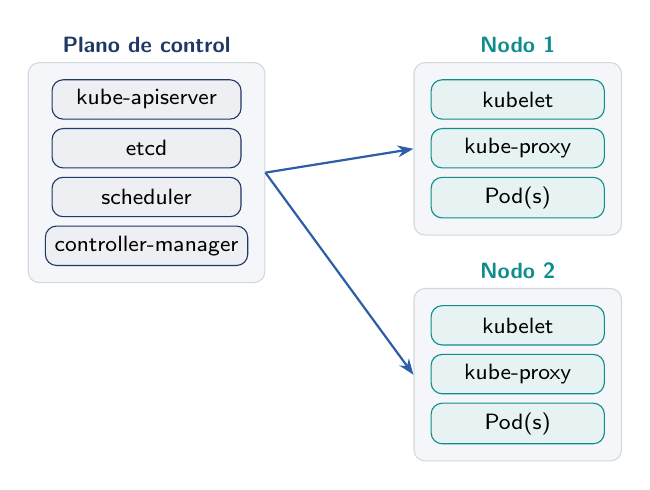
\begin{tikzpicture}[font=\footnotesize,
  cp/.style={draw=uteqBlue,fill=uteqBlue!8,rounded corners,minimum width=2.4cm,minimum height=0.5cm,align=center},
  nd/.style={draw=uteqTeal,fill=uteqTeal!10,rounded corners,minimum width=2.2cm,minimum height=0.5cm,align=center},
  box/.style={draw=grayLine,fill=grayBg,rounded corners,inner sep=6pt}]
% control plane
\node[cp] (api) {kube-apiserver};
\node[cp,below=3pt of api] (etcd) {etcd};
\node[cp,below=3pt of etcd] (sched) {scheduler};
\node[cp,below=3pt of sched] (cm) {controller-manager};
\begin{scope}[on background layer]
\node[box,fit=(api)(etcd)(sched)(cm),label={[uteqBlue]above:\bfseries Plano de control}] (cpbox) {};
\end{scope}
% node 1
\node[nd,right=2.4cm of api] (kubelet1) {kubelet};
\node[nd,below=3pt of kubelet1] (proxy1) {kube-proxy};
\node[nd,below=3pt of proxy1] (pod1) {Pod(s)};
\begin{scope}[on background layer]
\node[box,fit=(kubelet1)(proxy1)(pod1),label={[uteqTeal]above:\bfseries Nodo 1}] (n1) {};
\end{scope}
% node 2
\node[nd,below=1.1cm of pod1] (kubelet2) {kubelet};
\node[nd,below=3pt of kubelet2] (proxy2) {kube-proxy};
\node[nd,below=3pt of proxy2] (pod2) {Pod(s)};
\begin{scope}[on background layer]
\node[box,fit=(kubelet2)(proxy2)(pod2),label={[uteqTeal]above:\bfseries Nodo 2}] (n2) {};
\end{scope}
\draw[-{Stealth[length=2mm]},uteqMid,thick] (cpbox.east) -- (n1.west);
\draw[-{Stealth[length=2mm]},uteqMid,thick] (cpbox.east) -- (n2.west);
\end{tikzpicture}
\caption{Plano de control (decide) frente a nodos de trabajo (ejecutan). El \texttt{apiserver} es la \'unica puerta de entrada al cl\'uster.}
\label{fig:k8sarch}
\end{figure}

\textbf{Plano de control:} \texttt{kube-apiserver} (puerta de entrada \'unica; toda orden pasa por aqu\'i), \texttt{etcd} (almac\'en clave-valor que guarda el estado del cl\'uster), \texttt{scheduler} (decide en qu\'e nodo colocar cada Pod) y \texttt{controller-manager} (bucles que reconcilian estado real con estado deseado). \textbf{Nodo de trabajo:} \texttt{kubelet} (agente que arranca y vigila los Pods del nodo), \texttt{kube-proxy} (reglas de red para los Services) y un \emph{runtime} de contenedores (por ejemplo \texttt{containerd}).

\subsection{Objetos fundamentales}

\begin{description}[leftmargin=1.4em,style=nextline]
\item[Pod] la unidad m\'inima de despliegue: uno o varios contenedores que comparten red y almacenamiento. Los Pods son \emph{ef\'imeros}; no se gestionan directamente en producci\'on.
\item[ReplicaSet] garantiza que un n\'umero dado de r\'eplicas id\'enticas de un Pod est\'e siempre en ejecuci\'on.
\item[Deployment] gestiona ReplicaSets y a\~nade \emph{actualizaciones controladas} (rolling update) y \emph{rollback}. Es el objeto que el estudiante usar\'a para sus microservicios.
\item[Service] da una direcci\'on de red estable y balanceo a un conjunto cambiante de Pods, seleccionados por etiquetas. Tipos: \texttt{ClusterIP} (interno), \texttt{NodePort} (expone un puerto en cada nodo) y \texttt{LoadBalancer} (IP externa en la nube).
\item[ConfigMap / Secret] externalizan configuraci\'on y credenciales fuera de la imagen.
\item[Ingress] enruta tr\'afico HTTP externo hacia Services por host y ruta (el equivalente al gateway).
\end{description}

\subsection{Estructura de archivos del proyecto (etapa Kubernetes)}

\begin{lstlisting}[basicstyle=\ttfamily\footnotesize,numbers=none]
svc-estudiantes/
`-- k8s/
    |-- namespace.yaml       # aislamiento logico del proyecto
    |-- configmap.yaml       # configuracion no sensible
    |-- secret.yaml          # credenciales
    |-- deployment.yaml      # microservicio: 3 replicas + sondas
    |-- service.yaml         # IP estable + balanceo (ClusterIP)
    `-- ingress.yaml         # entrada HTTP externa (opcional)
\end{lstlisting}

\archivo{svc-estudiantes/k8s/deployment.yaml}
\begin{lstlisting}[language=yaml]
apiVersion: apps/v1
kind: Deployment
metadata:
  name: svc-estudiantes
  namespace: distapp
  labels:
    app: svc-estudiantes
spec:
  replicas: 3
  selector:
    matchLabels:
      app: svc-estudiantes
  template:
    metadata:
      labels:
        app: svc-estudiantes
    spec:
      containers:
        - name: svc-estudiantes
          image: svc-estudiantes:1.0.0
          ports:
            - containerPort: 8080
          envFrom:
            - configMapRef:
                name: svc-estudiantes-config
            - secretRef:
                name: svc-estudiantes-secret
          readinessProbe:
            httpGet:
              path: /actuator/health/readiness
              port: 8080
            initialDelaySeconds: 20
            periodSeconds: 10
          livenessProbe:
            httpGet:
              path: /actuator/health/liveness
              port: 8080
            initialDelaySeconds: 30
            periodSeconds: 15
          resources:
            requests:
              cpu: "250m"
              memory: "384Mi"
            limits:
              cpu: "1"
              memory: "768Mi"
\end{lstlisting}

\archivo{svc-estudiantes/k8s/service.yaml}
\begin{lstlisting}[language=yaml]
apiVersion: v1
kind: Service
metadata:
  name: svc-estudiantes
  namespace: distapp
spec:
  type: ClusterIP
  selector:
    app: svc-estudiantes      # enruta a todos los Pods con esta etiqueta
  ports:
    - port: 80                # puerto del Service
      targetPort: 8080        # puerto del contenedor
\end{lstlisting}

\archivo{svc-estudiantes/k8s/configmap.yaml}
\begin{lstlisting}[language=yaml]
apiVersion: v1
kind: ConfigMap
metadata:
  name: svc-estudiantes-config
  namespace: distapp
data:
  SPRING_PROFILES_ACTIVE: "docker"
  SPRING_DATASOURCE_URL: "jdbc:postgresql://postgres:5432/estudiantes"
\end{lstlisting}

\begin{keybox}[El contrato etiqueta-selector]
El \texttt{Service} no conoce IPs de Pods: declara un \texttt{selector} por etiqueta (\texttt{app: svc-estudiantes}) y K8s mantiene al d\'ia el conjunto de destinos. Este \emph{acoplamiento por etiquetas}, no por direcci\'on, es lo que permite escalar, reemplazar y desplegar Pods sin tocar la red. Tambi\'en es la palanca de los patrones blue-green y canary del subtema 4.
\end{keybox}

\subsection{Paso a paso en IntelliJ IDEA}

\begin{enumerate}
\item \textbf{Cl\'uster local.} Para practicar sin nube, instale \texttt{minikube} o \texttt{kind} y arr\'anquelo (\texttt{minikube start}). Esto genera un \texttt{kubeconfig} en \texttt{\textasciitilde/.kube/config}.
\item \textbf{Plugin Kubernetes.} En IntelliJ IDEA Ultimate viene incluido; en otras ediciones, inst\'alelo desde \emph{Settings} $\rightarrow$ \emph{Plugins}. Reconoce autom\'aticamente el \texttt{kubeconfig}.
\item \textbf{Aplicar manifiestos.} Abra cualquier \texttt{*.yaml} de \texttt{k8s/}: en el gutter aparece un icono para \emph{Apply} el recurso al cl\'uster. Tambi\'en puede arrastrar la carpeta completa.
\item \textbf{Explorar.} En \emph{Services} $\rightarrow$ \emph{Kubernetes} ver\'a \emph{Workloads} (Deployments, Pods), \emph{Network} (Services, Ingress) y \emph{Config} (ConfigMaps, Secrets). Doble clic en un Pod abre sus logs; \emph{Port Forward} expone el Service en \texttt{localhost} para probarlo.
\item \textbf{Editar en vivo.} El editor valida el esquema y autocompleta campos (\texttt{apiVersion}, \texttt{kind}), reduciendo errores de indentaci\'on YAML.
\end{enumerate}

\archivo{Terminal --- Windows PowerShell}
\begin{lstlisting}[numbers=none]
# Cargar la imagen local en minikube (sin registro remoto)
minikube image load svc-estudiantes:1.0.0

# Aplicar todos los manifiestos del directorio
kubectl apply -f k8s/

# Ver el estado de los objetos en el namespace
kubectl get pods,deploy,svc -n distapp

# Seguir el despliegue (rolling update) y leer logs
kubectl rollout status deployment/svc-estudiantes -n distapp
kubectl logs -f deploy/svc-estudiantes -n distapp

# Exponer el Service en localhost para probarlo
kubectl port-forward svc/svc-estudiantes 8080:80 -n distapp
\end{lstlisting}

% ===================================================================
\section{Subtema 4 --- Patrones de despliegue distribuido (blue-green y canary)}

\subsection{El problema: liberar sin tiempo de ca\'ida}

Actualizar un sistema distribuido en producci\'on plantea un dilema: detenerlo para cambiar la versi\'on viola el \textbf{SLA} de disponibilidad, pero cambiarlo en caliente arriesga propagar un fallo a todos los usuarios. Los \emph{patrones de despliegue} resuelven el dilema controlando \emph{qu\'e fracci\'on} del tr\'afico ve la versi\'on nueva y \emph{con qu\'e rapidez} se puede revertir \cite{richardson2018,newman2021}.

\subsection{Estrategia base de Kubernetes: rolling update}

Por defecto, un \texttt{Deployment} actualiza con \textbf{rolling update}: reemplaza los Pods viejos por nuevos de forma gradual, manteniendo siempre un m\'inimo disponible (\texttt{maxUnavailable}) y un m\'aximo de Pods extra (\texttt{maxSurge}). Es seguro y autom\'atico, pero mezcla ambas versiones durante la transici\'on y no permite ``probar con pocos usuarios antes de comprometerse''. Para eso existen blue-green y canary.

\subsection{Despliegue Blue-Green}

\begin{defbox}[Blue-Green]
Se mantienen \textbf{dos entornos id\'enticos}: \emph{blue} (versi\'on actual, recibe todo el tr\'afico) y \emph{green} (versi\'on nueva, desplegada en paralelo y verificada sin tr\'afico real). Cuando \emph{green} pasa las pruebas, se \textbf{conmuta el tr\'afico} de golpe (por ejemplo cambiando el \texttt{selector} del Service). Si algo falla, el \emph{rollback} es instant\'aneo: se vuelve a apuntar a \emph{blue}.
\end{defbox}

En Kubernetes se implementa con dos Deployments que comparten la etiqueta \texttt{app} pero difieren en \texttt{version}; el Service selecciona una sola versi\'on a la vez.

\archivo{svc-estudiantes/k8s/blue-green/service.yaml}
\begin{lstlisting}[language=yaml]
apiVersion: v1
kind: Service
metadata:
  name: svc-estudiantes
  namespace: distapp
spec:
  type: ClusterIP
  selector:
    app: svc-estudiantes
    version: blue            # <-- la palanca: cambiar a 'green' conmuta todo
  ports:
    - port: 80
      targetPort: 8080
\end{lstlisting}

\archivo{Terminal --- conmutaci\'on y rollback}
\begin{lstlisting}[numbers=none]
# 1) Desplegar green (version 1.1.0) en paralelo, sin trafico todavia
kubectl apply -f k8s/blue-green/deployment-green.yaml

# 2) Verificar green internamente (port-forward al Pod de green) ...

# 3) Conmutar TODO el trafico a green cambiando el selector del Service
kubectl patch service svc-estudiantes -n distapp `
  -p '{"spec":{"selector":{"app":"svc-estudiantes","version":"green"}}}'
# Linux/macOS: misma orden sin el backtick de continuacion

# 4) Rollback instantaneo si algo falla: volver a blue
kubectl patch service svc-estudiantes -n distapp `
  -p '{"spec":{"selector":{"app":"svc-estudiantes","version":"blue"}}}'
\end{lstlisting}

\textbf{Ventajas:} conmutaci\'on y rollback instant\'aneos; la versi\'on nueva se valida en un entorno id\'entico antes de recibir usuarios. \textbf{Desventajas:} duplica los recursos durante la transici\'on; un cambio de esquema de base de datos exige que ambas versiones sean compatibles con el mismo esquema.

\subsection{Despliegue Canary}

\begin{defbox}[Canary]
La versi\'on nueva (\emph{canary}) recibe un \textbf{peque\~no porcentaje} del tr\'afico real (por ejemplo 10\,\%) mientras la \emph{stable} atiende el resto. Se observan m\'etricas (errores, latencia); si el canary se comporta bien, se incrementa su proporci\'on de forma progresiva hasta el 100\,\%; si no, se retira afectando solo a una minor\'ia de usuarios. El nombre alude al ``canario en la mina''.
\end{defbox}

La forma m\'as simple en K8s vanilla es jugar con el \emph{n\'umero de r\'eplicas}: un Service que selecciona la etiqueta com\'un \texttt{app} reparte tr\'afico proporcionalmente entre Pods stable y canary. Para control fino de porcentajes independiente del conteo de Pods se usan pesos de \texttt{Ingress} (anotaciones de canary) o herramientas como \emph{Argo Rollouts}.

\begin{figure}[h]
\centering
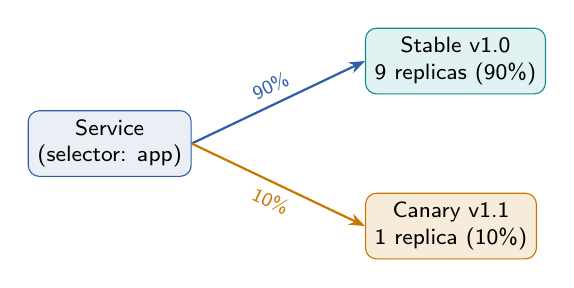
\begin{tikzpicture}[font=\footnotesize,
  n/.style={draw,rounded corners,minimum width=2.0cm,minimum height=0.6cm,align=center}]
\node[n,draw=uteqMid,fill=uteqMid!10] (svc) {Service\\(selector: app)};
\node[n,draw=uteqTeal,fill=uteqTeal!12,above right=0.2cm and 2.2cm of svc] (stable) {Stable v1.0\\9 replicas (90\%)};
\node[n,draw=uteqAmber,fill=uteqAmber!15,below right=0.2cm and 2.2cm of svc] (canary) {Canary v1.1\\1 replica (10\%)};
\draw[-{Stealth[length=2mm]},uteqMid,thick] (svc.east) -- node[above,sloped,font=\scriptsize]{90\%} (stable.west);
\draw[-{Stealth[length=2mm]},uteqAmber,thick] (svc.east) -- node[below,sloped,font=\scriptsize]{10\%} (canary.west);
\end{tikzpicture}
\caption{Canary por r\'eplicas: el Service reparte el tr\'afico en proporci\'on al n\'umero de Pods de cada versi\'on que comparten la etiqueta \texttt{app}.}
\label{fig:canary}
\end{figure}

\archivo{svc-estudiantes/k8s/canary/deployment-canary.yaml}
\begin{lstlisting}[language=yaml]
apiVersion: apps/v1
kind: Deployment
metadata:
  name: svc-estudiantes-canary
  namespace: distapp
  labels:
    app: svc-estudiantes      # MISMA etiqueta 'app' que stable -> el Service lo incluye
    track: canary
spec:
  replicas: 1                 # 1 de 10 Pods totales ~= 10% del trafico
  selector:
    matchLabels:
      app: svc-estudiantes
      track: canary
  template:
    metadata:
      labels:
        app: svc-estudiantes
        track: canary
    spec:
      containers:
        - name: svc-estudiantes
          image: svc-estudiantes:1.1.0
          ports:
            - containerPort: 8080
\end{lstlisting}

\begin{table}[h]
\centering
\caption{Comparaci\'on de estrategias de despliegue distribuido.}
\label{tab:estrategias}
\small
\begin{tabularx}{\linewidth}{@{}l C C C@{}}
\toprule
\textbf{Criterio} & \textbf{Rolling update} & \textbf{Blue-Green} & \textbf{Canary} \\
\midrule
Tiempo de ca\'ida & Cero & Cero & Cero \\
Coste de recursos & Bajo & Alto (doble) & Medio \\
Velocidad de rollback & Media & Instant\'anea & Alta \\
Exposici\'on al riesgo & Gradual & Total al conmutar & M\'inima (pocos usuarios) \\
Prueba con tr\'afico real & No selectiva & No (antes de conmutar) & S\'i, controlada \\
Complejidad & Baja (nativa) & Media & Alta (m\'etricas) \\
\bottomrule
\end{tabularx}
\end{table}

\begin{warnbox}[Regla de oro para ambos patrones]
Toda liberaci\'on progresiva exige \textbf{compatibilidad hacia atr\'as}: mientras dos versiones conviven, deben tolerar el mismo esquema de datos y el mismo contrato de API. Los cambios de esquema se hacen en pasos \emph{aditivos} (expand) antes de eliminar lo viejo (contract).
\end{warnbox}

% ===================================================================
\section{Cierre, actividad y evaluaci\'on}

\subsection{Actividad de clase sugerida}

Sobre el microservicio \texttt{svc-estudiantes}, el estudiante debe: (1) escribir el \texttt{Dockerfile} multi-etapa y construir la imagen desde IntelliJ; (2) levantar el stack con \texttt{compose.yaml} (microservicio + PostgreSQL + Nginx) y probar un flujo \texttt{POST}/\texttt{GET} v\'ia gateway; (3) desplegar el \texttt{Deployment} y el \texttt{Service} en minikube y comprobar 3 r\'eplicas sanas; y (4) ejecutar una conmutaci\'on blue-green y un canary de 1 r\'eplica, documentando con capturas el estado antes y despu\'es. Entregable: repositorio con \texttt{Dockerfile}, \texttt{compose.yaml}, carpeta \texttt{k8s/} y un \texttt{README.md} reproducible.

\subsection{Preguntas de comprobaci\'on y defensa}

\begin{enumerate}
\item \textbf{Conceptual:} ¿Por qu\'e un contenedor arranca en milisegundos y una VM en decenas de segundos? Relacione la respuesta con la Figura~\ref{fig:vmvscont}.
\item \textbf{Dise\~no:} En el \texttt{Dockerfile}, ¿qu\'e gana exactamente la etapa de runtime al usar \texttt{eclipse-temurin:25-jre-alpine} en vez de \texttt{25-jdk}? Cuantif\'iquelo.
\item \textbf{Compose:} ¿Por qu\'e la aplicaci\'on se conecta a la base de datos usando el host \texttt{db} y no \texttt{localhost}? ¿Qu\'e mecanismo lo hace posible?
\item \textbf{Kubernetes:} Si un Pod del Deployment muere, ¿qu\'e componente lo detecta y qu\'e objeto garantiza que vuelva a haber 3 r\'eplicas?
\item \textbf{Service:} Explique por qu\'e el \texttt{Service} no necesita conocer las IPs de los Pods. ¿Qu\'e papel cumple el \texttt{selector}?
\item \textbf{Patrones:} Un equipo libera v1.1 y descubre un fallo grave 30 segundos despu\'es. ¿Qu\'e estrategia le da el rollback m\'as r\'apido: blue-green o canary? Justifique.
\item \textbf{Cr\'itica:} ¿Por qu\'e ambos patrones exigen compatibilidad de esquema de base de datos entre versiones? D\'e un ejemplo de cambio que rompa la convivencia.
\end{enumerate}

\begin{thebibliography}{9}
\footnotesize
\bibitem{merkel2014} D. Merkel, ``Docker: lightweight Linux containers for consistent development and deployment,'' \emph{Linux Journal}, vol. 2014, no. 239, art. 2, Mar. 2014.
\bibitem{bernstein2014} D. Bernstein, ``Containers and cloud: From LXC to Docker to Kubernetes,'' \emph{IEEE Cloud Computing}, vol. 1, no. 3, pp. 81--84, Sep. 2014, doi: 10.1109/MCC.2014.51.
\bibitem{pahl2019} C. Pahl, A. Brogi, J. Soldani, and P. Jamshidi, ``Cloud container technologies: A state-of-the-art review,'' \emph{IEEE Transactions on Cloud Computing}, vol. 7, no. 3, pp. 677--692, Jul.--Sep. 2019, doi: 10.1109/TCC.2017.2702586.
\bibitem{burns2016borg} B. Burns, B. Grant, D. Oppenheimer, E. Brewer, and J. Wilkes, ``Borg, Omega, and Kubernetes,'' \emph{Communications of the ACM}, vol. 59, no. 5, pp. 50--57, May 2016, doi: 10.1145/2890784.
\bibitem{hightower2022} B. Burns, J. Beda, K. Hightower, and L. Evenson, \emph{Kubernetes: Up and Running}, 3rd ed. Sebastopol, CA, USA: O'Reilly Media, 2022. ISBN: 978-1-098-11020-8.
\bibitem{burns2025} B. Burns, \emph{Designing Distributed Systems}, 2nd ed. Sebastopol, CA, USA: O'Reilly Media, 2025. ISBN: 978-1-09-815635-0.
\bibitem{richardson2018} C. Richardson, \emph{Microservices Patterns: With Examples in Java}. Shelter Island, NY, USA: Manning Publications, 2018. ISBN: 978-1-617-29454-1.
\bibitem{newman2021} S. Newman, \emph{Building Microservices: Designing Fine-Grained Systems}, 2nd ed. Sebastopol, CA, USA: O'Reilly Media, 2021. ISBN: 978-1-4920-3402-5.
\bibitem{guerrero2026} G. C. Guerrero Ulloa, \emph{Aplicaciones Distribuidas: Notas de Curso}, Cap. 7. Quevedo, Ecuador: UTEQ, 2026.
\end{thebibliography}

\end{document}
